\documentclass[conference]{IEEEtran}
\usepackage{hyperref}
\usepackage{amsmath,amssymb,amsfonts}
\usepackage{algorithmic}
\usepackage{graphicx}
\usepackage{textcomp}
\usepackage{xcolor}
\def\BibTeX{{\rm B\kern-.05em{\sc i\kern-.025em b}\kern-.08em
    T\kern-.1667em\lower.7ex\hbox{E}\kern-.125emX}}

\usepackage[backend=biber,sorting=none]{biblatex}
\addbibresource{refs.bib}

\begin{document}

\title{
	On the bang sensor networks for ``BangNet'': \\
	Synchronised timestamps \& firmware updates
}

\author{
	\IEEEauthorblockN{Ted Johnson, Team ESP32resso}
	\IEEEauthorblockA{
		\textit{School of Computer Science \& Statistics} \\
		\textit{Trinity College Dublin (TCD)}\\
		Dublin, Ireland \\
		Email: edjohnso@tcd.ie
	}
}
\maketitle

\begin{abstract}
As part of our BangNet project, in which we attempt to catch wildfires early by pinpointing lightning strikes using networks of low-cost wireless microphones, we face a number of significant technical challenges. Included in these is the ability to quickly collect synchronised thunderclap timestamps and perform microcontroller firmware updates in highly remote environments. In this document, I first describe the overall technical design of BangNet and present my four main contributions to overcome these challenges. This is followed by a breakdown and analysis of the design choices made for each solution, including consideration of alternatives and resolution of encountered issues. Finally, I conclude with a summary of the work done so far as well as a brief reflection on my experience.
\end{abstract}

\begin{IEEEkeywords}
Internet of Things, LoRa, time synchronisation, over-the-air updates, multilateration.
\end{IEEEkeywords}



\section{Introduction}

The BangNet project is our effort to catch and prevent lightning strikes from igniting and spreading into catastrophic wildfires within susceptible regions, such as California and Australia. In the United States, at least 3,790 fatalities have been attributed to wildfires in the 2022, with suppression of wildfires are estimated to cost the taxpayer on average \$3 billion each year\cite{fire-stats}. Additionally, it is reported that lightning is the most common source of ignition, above any other natural causes and human activity\cite{fire-cause}. As such, we believe the BangNet project is a particularly suitable use of Internet of Things (IoT) technology and can provide significant value to society.

To accomplish this goal, we have designed a system capable of quickly identifying the location of a lightning strike by analysing the arrival time difference of its thunderclap sound wave across various microphones scattered within a region. This is made possible using a technique called pseudo-range multilateration (MLAT), or more specifically acoustic location by time difference of arrival (TDoA)\cite{mlat-tdoa}, as seen in Fig.~\ref{trilateration_figure}. This method has been used throughout recent history, most notably in locating enemy military artillery batteries, where it is called sound ranging\cite{sound-ranging}. We then use this information to drive servomotors such that attached visual and thermal imaging cameras can capture images of the suspected fire. These images can be processed for the presence of smoke and fire, in which case authorities can be immediately alerted of the potential wildfire. However, this final step of image processing has been set as outside the scope of our project given the time constraint. A diagram of the system architecture can be viewed in Fig.~\ref{architecture_figure}. This report will focus entirely on the design and implementation of the bang sensor network component, found on the left-hand side of Fig.~\ref{architecture_figure} as step 1 to 2.

\begin{figure}[ht]
\centerline{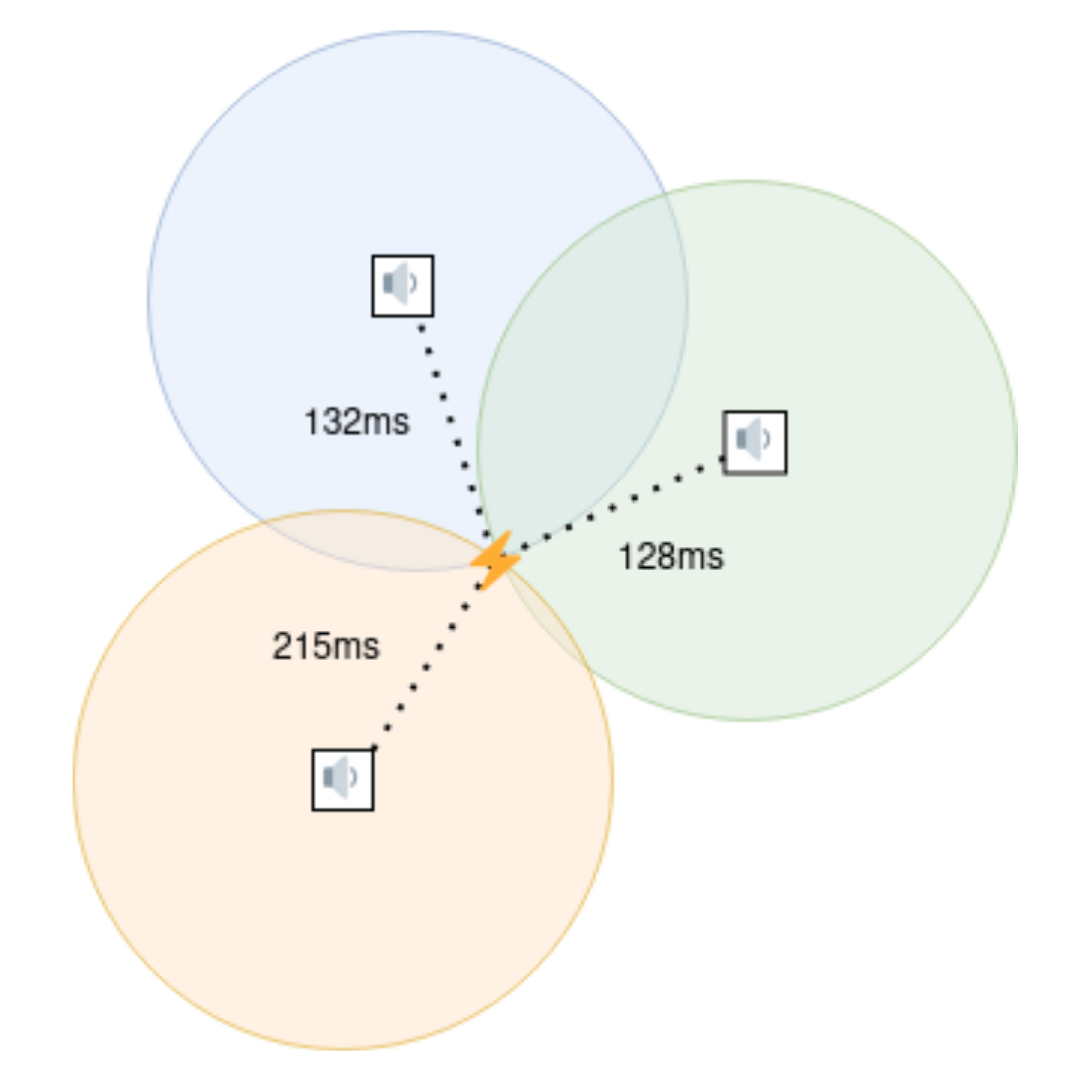
\includegraphics[width=80mm]{images/trilateration.png}}
\caption{Use of MLAT to locate lightning strike with thunder TDoA}
\label{trilateration_figure}
\end{figure}

In order for our system to be effective, we must rapidly compile a series of precise and accurate thunderclap timestamps from several distributed locations. This necessitates that our microphones be placed far apart while maintaining a common understanding of the current time. Furthermore, these networks of sensors are most likely to be deployed in highly remote environments, namely throughout expansive bushlands and savannas. As such, we cannot expect every device to have access to the infrastructure required for an electric power source or Internet access through a Wi-Fi connection. Instead, upon detecting thunder, these remote sensors record their current time and broadcast it to other sensors. Nearby sensors connected to the Internet receive these timestamps and relay to our cloud application where they are compiled as input for MLAT. This situation is an ideal application for the LoRa radio communication technique, which capabilities can provide greater than 10 kilometer range data transmission on low-powered devices. To balance this, it has a very limited bitrate, generally achieving less than 50 kilobits per second. As our primary communication requirements are remote sensors irregularly sending single timestamps consisting of 64 bits, we accept this drawback.

\begin{figure}[ht]
\centerline{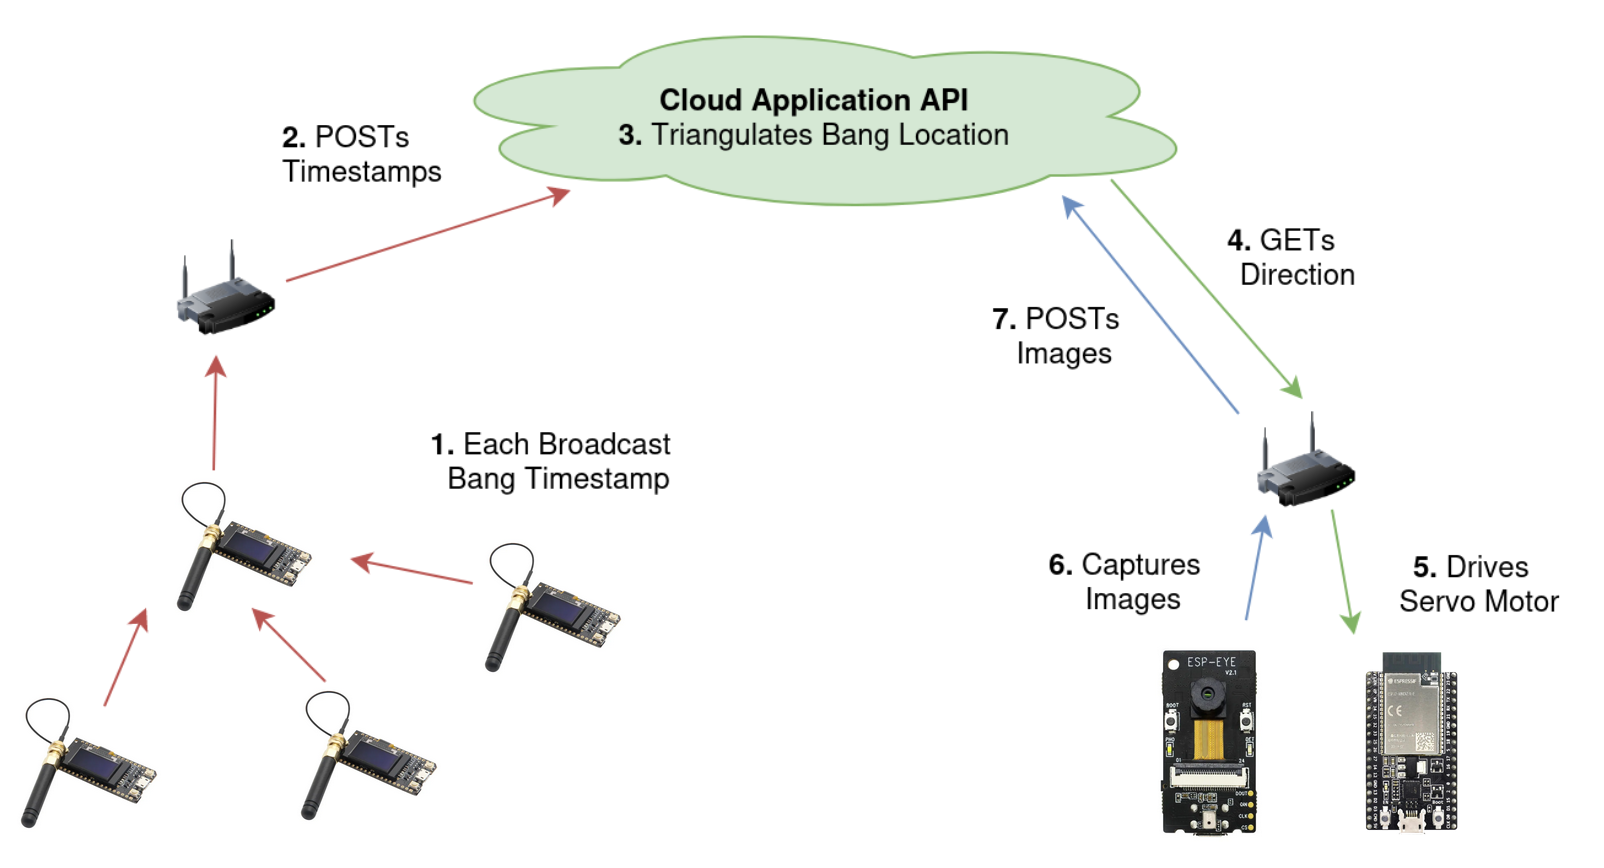
\includegraphics[width=90mm]{images/architecture.png}}
\caption{System architecture diagram for BangNet, consisting the bang sensor networks on the left, our cloud application at the top and the servomotor imaging devices on the right}
\label{architecture_figure}
\end{figure}

When organising responsibility for tasks amongst our team, I was elected to work on both the microcontroller firmware and optimising the software development process. Over the course of the project, I specialised in the firmware build processes, overall architecture and over-the-air updates, bang sensor time synchronisation and the LoRa communication protocol. To discuss the design decisions I made during my work, I have divided this essay into the following four sections:

\paragraph{\nameref{architecture}} To begin, there is a explanation of our firmware architecture and how we access the flexibility of the Arduino framework without sacrificing any functionality of ESP-IDF.
\paragraph{\nameref{synchronisation}} A comparison of the different approaches to time synchronisation we considered is given, followed by a description of our solution.
\paragraph{\nameref{updates}} I present our secure remote firmware updating method based on delta encoding, binary patching and signed app verification.
\paragraph{\nameref{lora}} In this final section, the above systems are tied together under the communication protocol we use to exchange data between the constrained bang sensor devices with LoRa.

I finish with a summary of the work completed thus far, followed by a short reflection on my experience during this project.



\section{Firmware Architecture} \label{architecture}

As a member of both the software development process and firmware groups, one of the earliest tasks I worked on was investigating how we should build and flash firmware to each of our devices. For instance, we need to be able to compile the bang sensor code such that it could be executed on the LILYGO LoRa32 v1.0, Heltek WiFi LoRa 32 V1 and Heltek WiFi LoRa 32 V1. Additionally, we wanted to choose a development framework we would base our application on top of that would minimise the effort needed to implement features and allow us to interface with community libraries while providing us with access to all required board functionality. Later, I would also contribute the overall software architecture we would use to structure our applications in a logical manner without compromising performance. In the following sections, I will go into detail on each of these topics and provide some insight into our reasoning on our development decisions.

\subsection{PlatformIO and the Arduino Framework}

Initially, we found PlatformIO to be particularly promising build tool, as it abstracts away a lot of the boilerplate code and headaches incurred from developing for heterogeneous boards. Similarly, we could use it to compile code for the Arduino framework, which significantly reduces the learning curve for us to get started with microcontroller programming and has a highly active surround community providing comprehensive documentation and a huge collection of supported libraries. With these tools, we were able to produce and test our first functional firmware for the sensor devices within only a few hours.

However, it soon became obvious that neither PlatformIO nor the Arduino framework would not be sufficient for our needs. Most critically, the Arduino framework provided through PlatformIO uses a pre-compiled ESP-IDF library which prevents any configuration of ESP-IDF build time options. Included in these are the options to enable and use Signed App Verification on boot and after performing a firmware update. Without this, it would become infeasible for us to implement a secure procedure for updating firmware over the network, as discussed in Section \ref{updates}. As such, to access all required board functionality, it was necessary to dispose of PlatformIO as an abstraction of the build process and instead use ESP-IDF directly.

\subsection{ESP-IDF and the Arduino Framework}

While using ESP-IDF offers much greater control over the build process and allows us full access to all ESP32 functionality, it comes at the cost of increased installation, development and build complexity. Moreover, we lose all of the benefits from using the Arduino framework as the ESP-IDF framework has considerably less community support and presents a much harder challenge to program for. In table \ref{build_tool_table}, I have presented a number of approximate metrics we used when comparing the developer experience of using the ESP-IDF toolchain over using the PlatformIO build tool with the Arduino framework.

\begin{table}[ht]
\caption{Comparison Of Build Tool Developer Experience}
\begin{center}
\begin{tabular}{|c|c|c|}
\hline
& \textbf{PlatformIO} & \textbf{ESP-IDF} \\
\hline
Hours to setup from zero-knowledge & \textit{0.5} & \textit{7.5} \\
\hline
Lines in project configuration file & \textit{10} & \textit{2117} \\
\hline
Lines in minimal Wi-Fi example code & \textit{16} & \textit{172} \\
\hline
Mean seconds to compile example code & \textit{10.5} & \textit{54.3} \\
\hline
Open-source libraries available\cite{pio-libraries}\cite{idf-libraries} & \textit{9351} & \textit{314} \\
\hline
\end{tabular}
\label{build_tool_table}
\end{center}
\end{table}


Evidently, it would be most preferable if we were able to access the flexibility offered to us by the Arduino framework through its large community support while still retaining the required control over the build process needed to access all ESP-IDF functionality. Fortunately, after searching for solutions, we found that this is possible through including the Arduino framework and community libraries as ESP-IDF components. These third-party projects must be defined properly within CMake, which allows the ESP-IDF build tool to configure, compile and link them together into the final binary. We can then include these into our own code like we would system libraries.


\subsection{FreeRTOS}

In our project's planned deployment scenario, most remote sensor devices would be entirely reliant on a single set of batteries for power and would therefore be highly constrained in power consumption if they were to have sufficient lifespans. As such, it is necessary for us to avoid idle loops and continuous polling as well as enforcing graceful device rebooting in the event of malfunction as opposed to entering a state of boot-loop. This is achieved through usage of FreeRTOS to orchestrate asynchronous execution of independent tasks, each yielding execution to the FreeRTOS runtime environment while idle, such as waiting for network IO, synchronisation primitives or timers. During such periods, it is possible for the device to enter sleep modes to conserve power.

In order to greatly simplify the design, development and reasoning about multiple FreeRTOS tasks executing in parallel, an architecture pattern was conceived that tasks should generally wait on a single input source, such as messages from other tasks or the expiry of a timer, then perform some operations and potentially output messages to other tasks before returning to waiting for the next input. Following this, we found that FreeRTOS queues fulfill the exact functionality needed to safely pass these messages between tasks. This had the added benefit of allowing tasks to idly wait on the production of new messages from many other tasks without requiring large amounts of shared global state complete with complex synchronisation logic which could easily introduce risks such as deadlock or invalid state representation.

Figure \ref{firmware_figure} provides a high-level overview of how this architecture pattern is implemented for bang sensor network devices. Notice that every sensor device can either be operating as a gateway sensor or a remote sensor depending on if a Wi-Fi connection could be established, where a remote sensor communicates only over LoRa, while gateway sensors can then relay with our cloud application using Wi-Fi. Therefore, the same firmware is used for both remote and gateway sensor devices but different sets of FreeRTOS tasks are instantiated for each.

\begin{figure}[ht]
\centerline{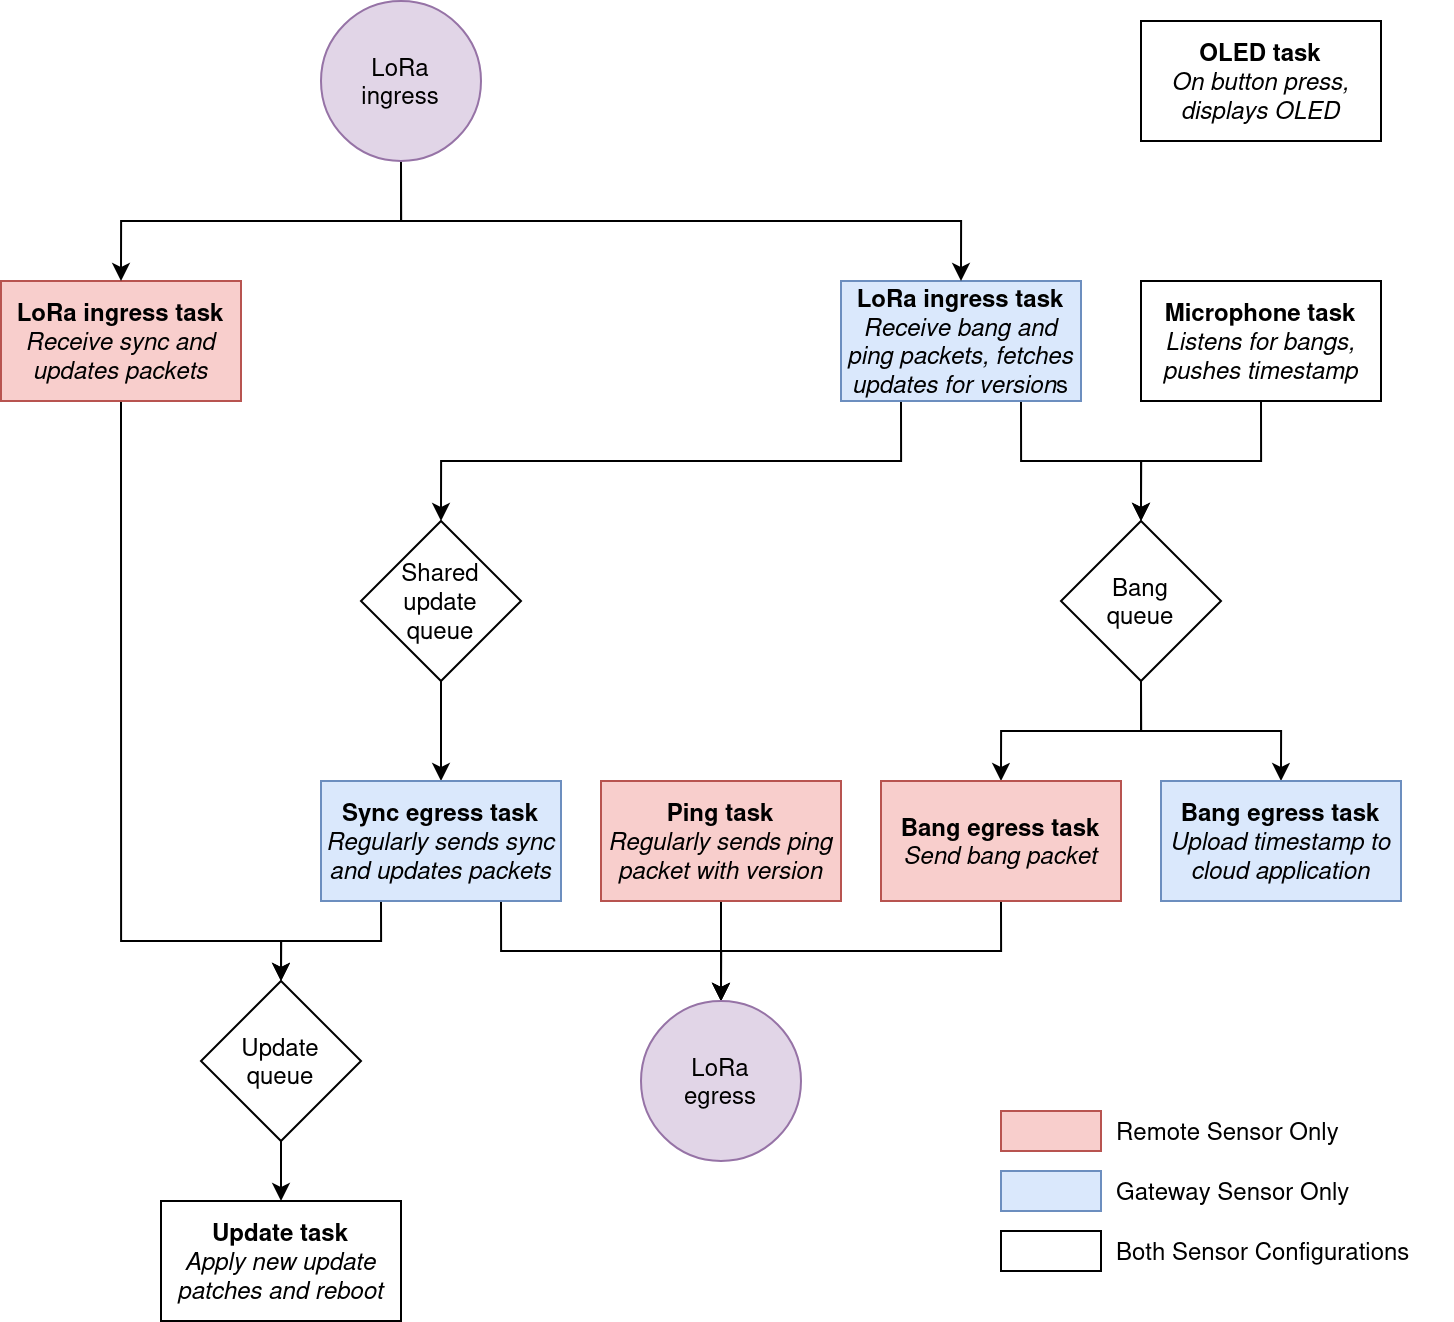
\includegraphics[width=90mm]{images/firmware.png}}
\caption{Illustration of how the firmware architecture for sensor devices is divided into a number of dedicated asynchronous tasks using queue-based communication for exchange of relevant data}
\label{firmware_figure}
\end{figure}

As FreeRTOS is highly customisable in functionality for the desired application, there are a number of complexities that we have not had the opportunity to investigate. One notable potential improvement to reduce our overall power consumption is configuring FreeRTOS to operate in a tickless kernel mode, where instead of regularly waking the device to test for timer expiry, interrupts are only raised by timers once a timer has expired. It is also possible for us to optimise our application in a number of aspects, such as lowering our device clock frequency and minimising the stack sizes allocated to each FreeRTOS process. However, as we are limited in the amount of time we can dedicate to this project, we have prioritised other areas that require more work.

\section{Time Synchronisation} \label{synchronisation}

One difficult aspect of BangNet is the requirement that all sensor devices need to maintain some common time reference so that an accurate TDoA between all sensors can be the determined for input to MLAT. Increased deviation in time reference between devices results in decreased accuracy of our lightning strike position estimation. By introducing noise to the time references of 5 sensors in a simulated environment, we were able to produce figure \ref{precision_figure} which shows that an error of 10 milliseconds between devices can emit positioning errors of up to 3 metres. In general, we saw that for every 1 millisecond of time reference error, we should expect a mean positioning error of 16.67 centimetres with a standard deviation of 7 centimetres.

\begin{figure}[ht]
\centerline{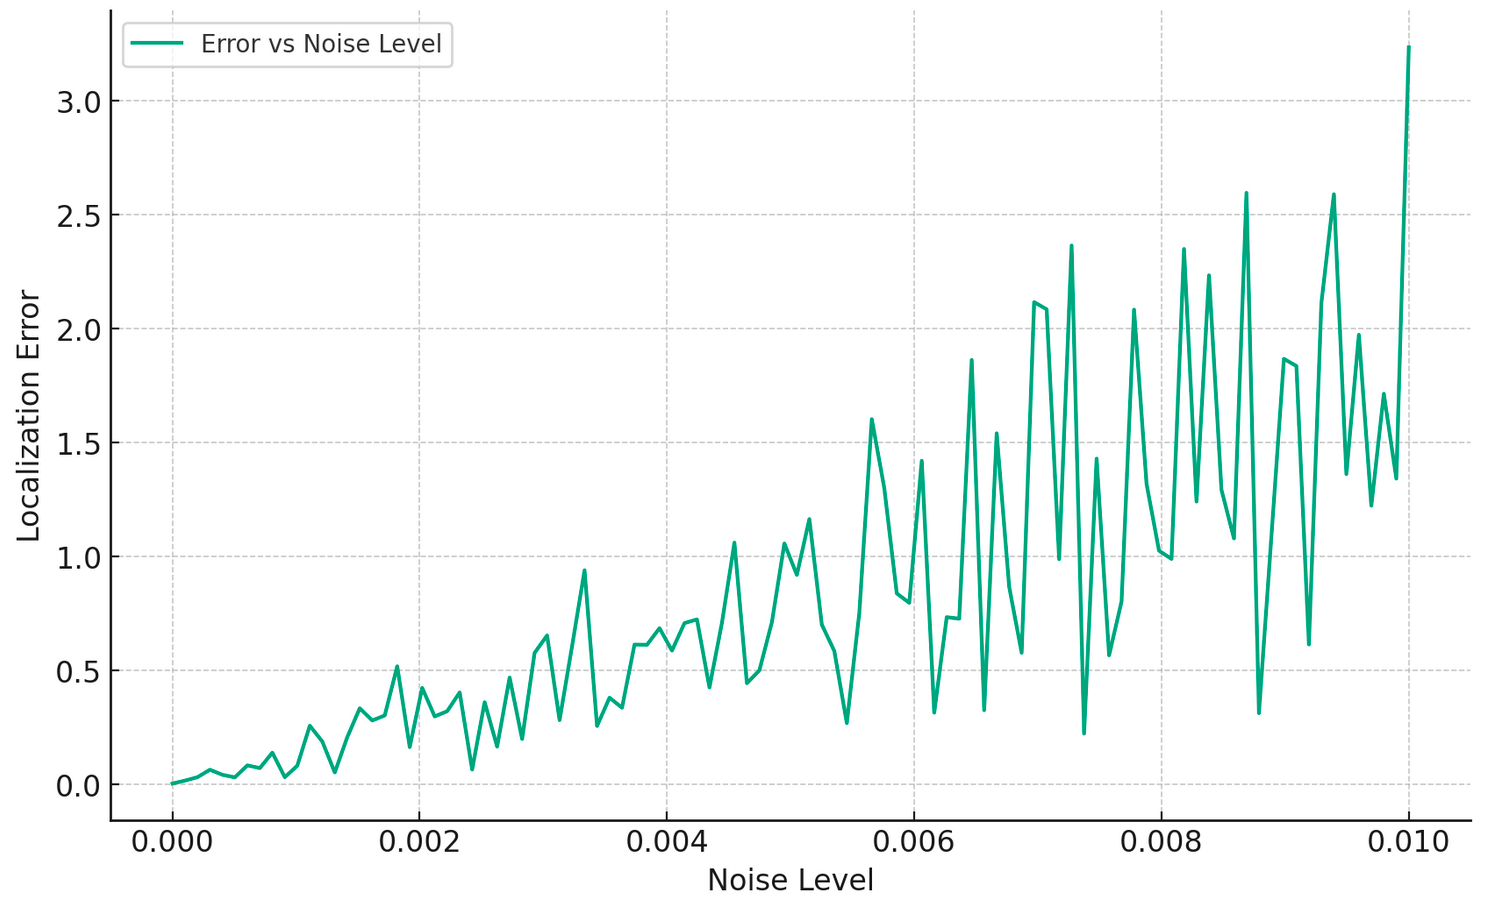
\includegraphics[width=90mm]{images/precision.png}}
\caption{Plot of TDoA noise in seconds against MLAT localisation error in metres when using 5 sensors in a simulated environment}
\label{precision_figure}
\end{figure}

From this, we can find that that if we want to achieve an average accuracy of within 15 metres using 5 sensors, we need to gain a precision of under 90 milliseconds between all sensors. To accomplish this, we investigated a number of approaches to compare their reported precision, ease-of-use and power consumption, as well as any other benefits and limitations associated with the method\cite{sync-methods}.

\paragraph{Network Time Protocol (NTP)} NTP is used in abundance to synchronise clocks across the Internet. Fundamentally, it functions by allowing systems to query a hierarchy of time servers with the intersection algorithm, which works to overcome the effects of network latency\cite{rfc1305}. As the gateway sensor device is directly connected to the Internet, it could regularly send an NTP packet over UDP to an appropriate time server as pointed to by http://pool.ntp.org. Upon receiving an NTP packet response containing the time references when the time server received the request and sent the response, a simplified implementation of the intersection algorithm can be used to attempt to subtract the effect of variable network latency. This timing information can then be broadcasted once over LoRa to all remote sensor devices, allowing all to receive this packet within less than a millisecond of each other.

\paragraph{Global Positioning System (GPS)} As part of GPS, each satellite transmits highly accurate and precise timing information. This has the additional benefit of providing geo-positioning data to the sensor, which could eliminate the need for operators to manually input such data. On the other hand, sensor devices would need to be equipped with their own GPS receiver, which would significantly increase power consumption and cost. Devices would also need a clear line of sight with the sky, but this should be expected in our deployment scenario but does add a limitation. The same approach as NTP of having only gateway sensor devices declare the time could again be used here to reduce the effect of many of these caveats, but this would necessitate a conscience decision to install GPS receivers only on devices to be used as gateways with the firmware somehow capable of detecting this and reacting accordingly.

\paragraph{The Things Network (TTN)} TTN downlink messages embed timing information in their payload field. As all of our sensor devices already use LoRa for communication, no additional hardware would be needed to start using TTN. However, this methodology would require conformation with the LoRaWAN protocol and be entirely reliant on the presence of third-party TTN servers. Moreover, TTN downlink messages are not to be part of regular communication and are subject to harsh usage restrictions. It would be expected to receive less than 10 in a 24-hour period. As such, devices would quickly fall out of synchronisation during the day.

\begin{table}[ht]
\caption{Comparison of Time Synchronisation Techniques}
\begin{center}
\begin{tabular}{|c|c|c|c|c|}
\hline
\textbf{Method} & \textbf{Precision} & \textbf{Power Draw} & \textbf{Cost} & \textbf{Requirements} \\
\hline
\textit{NTP} & \textless 100 ms & \textless 1mA & None & Internet connection \\
\hline
\textit{GPS} & \textless 10 ms & \textgreater 30mA & \textgreater 10€ & GPS reception \\
\hline
\textit{TTN} & \textgreater 100 ms & \textless 1mA & None & TTN servers \\
\hline
\end{tabular}
\label{synchronisation_table}
\end{center}
\end{table}

Considering the approximate specifications for each approach with found in table \ref{synchronisation_table}, we have chosen to implement the NTP solution for our project. As a time reference, we use the number of microseconds since 1900 encoded as a 64 bit unsigned integer. We don't believe the increased power consumption and overall project complexity is worth the higher precision of using GPS receivers, as we already require an Internet connection and NTP can deliver enough precision to match our requirements.




\section{Over-The-Air Updates} \label{updates}

Another significant challenge we set ourselves in this project was to allow the firmware of devices to be updated securely without physical access. In our deployment scenario, we assume many of these devices could be in highly remote environments where it would be impractical for operators to retrieve to perform firmware updates. Instead, devices should be able to receive and apply updates to themselves. Importantly, devices should also be able to validate the integrity and authenticity of the update before accepting it so that neither network corruption nor malicious parties can inject arbitrary instructions into the devices.

\subsection{ESP32 OTA}

Fortunately, the ESP32 framework provides all the functionality required to implement over-the-air updates (OTA) with just a few functions to start the update, write a part of the update and finish the update. To enable support for OTA, the device's partition table must be configured to include two OTA application slots. This allows one of the partitions to be updated with the contents of the new firmware while the other partition is still under execution. Then, once the update is completed successfully, the bootloader can be changed to boot the updated partition and the device is rebooted. If any issues occur, the original partition can continue to be executed while the updated partition is reverted. In this way, the device remains functional in all cases.

\subsection{Delta Encoding}

Without specialised logic, the ESP32 OTA functions expect to receive an entire copy of the new firmware binary in many parts which are used to completely overwrite the partition to be updated. However, this is infeasible if we plan to transmit updates over LoRa as the firmware binary is several megabytes in size but we expect to only be able to transmit less than a kilobyte of data per second. Furthermore, we will not be using any form of acknowledgements nor retransmission due to the extremely tight bandwidth and duty cycle restrictions of LoRa so if a single packet is missed or if forward-error correction cannot account for errors, we have to wait for the next opportunity to perform OTA.

One technique we can use to drastically reduce the amount of data needed to be transmitted is to send only the difference between the current firmware and the new firmware. Then, the device can use this difference to patch the current firmware. This is highly effective at reducing bandwidth usage and is already used by a number of projects, such as Google Chrome\cite{chrome-delta-updates}. Before we can generate a binary difference for a device, we first need know what firmware is already present. In this project, we have every device regularly `ping' a message containing their current firmware version. Once the cloud application receives this via the gateway device, it can generate an appropriate binary difference to broadcast back into the sensor network. This process can be seen through steps 1 to 4 in figure \ref{updates_figure}.

\begin{table}[ht]
\caption{Considered Binary Differencing Algorithms}
\begin{center}
\begin{tabular}{|c|c|}
\hline
\textbf{Algorithm} & \textbf{Source URL}\\
\hline
\textit{detools} & https://github.com/eerimoq/detools \\
\hline
\textit{HDiffPatch} & https://github.com/sisong/HDiffPatch \\
\hline
\textit{xdelta} & https://github.com/jmacd/xdelta \\
\hline
\textit{bsdiff} & https://github.com/mendsley/bsdiff \\
\hline
\end{tabular}
\label{difference_table}
\end{center}
\end{table}

In table \ref{difference_table}, I have compiled a list of prominent binary differencing algorithms commonly used today. We are still investigating which algorithm is the optimal choice for our project based on the estimated binary data savings, executable size of the patching library to be included on all devices and ease-of-use for generating and applying patches. We hope to have completed our implementation within the remaining project time frame.

\subsection{Signed App Verification}

We chose to use public key cryptography to ensure update integrity and authenticity. As illustrated in figure \ref{updates_figure}, every device includes our public key in their bootloader and all firmware updates are signed with our private key. This signature is included within the firmware update. Then, after the update procedure has been completed as outlined in the above sections, the public key is used to verify the updates signature against the updated partition using a feature of the ESP32 framework called Signed App Verification. The process will reject the firmware update if the signature is invalid to the public key or does not match the updated partition. Note that this does not prevent modification of the firmware through physical access, but we have decided to place this outside of the scope of the project. If we were to pursue this functionality, we could make use of ESP32 Secure Boot and Flash Encryption to ensure only our code can execute on the device.

\begin{figure}[ht]
\centerline{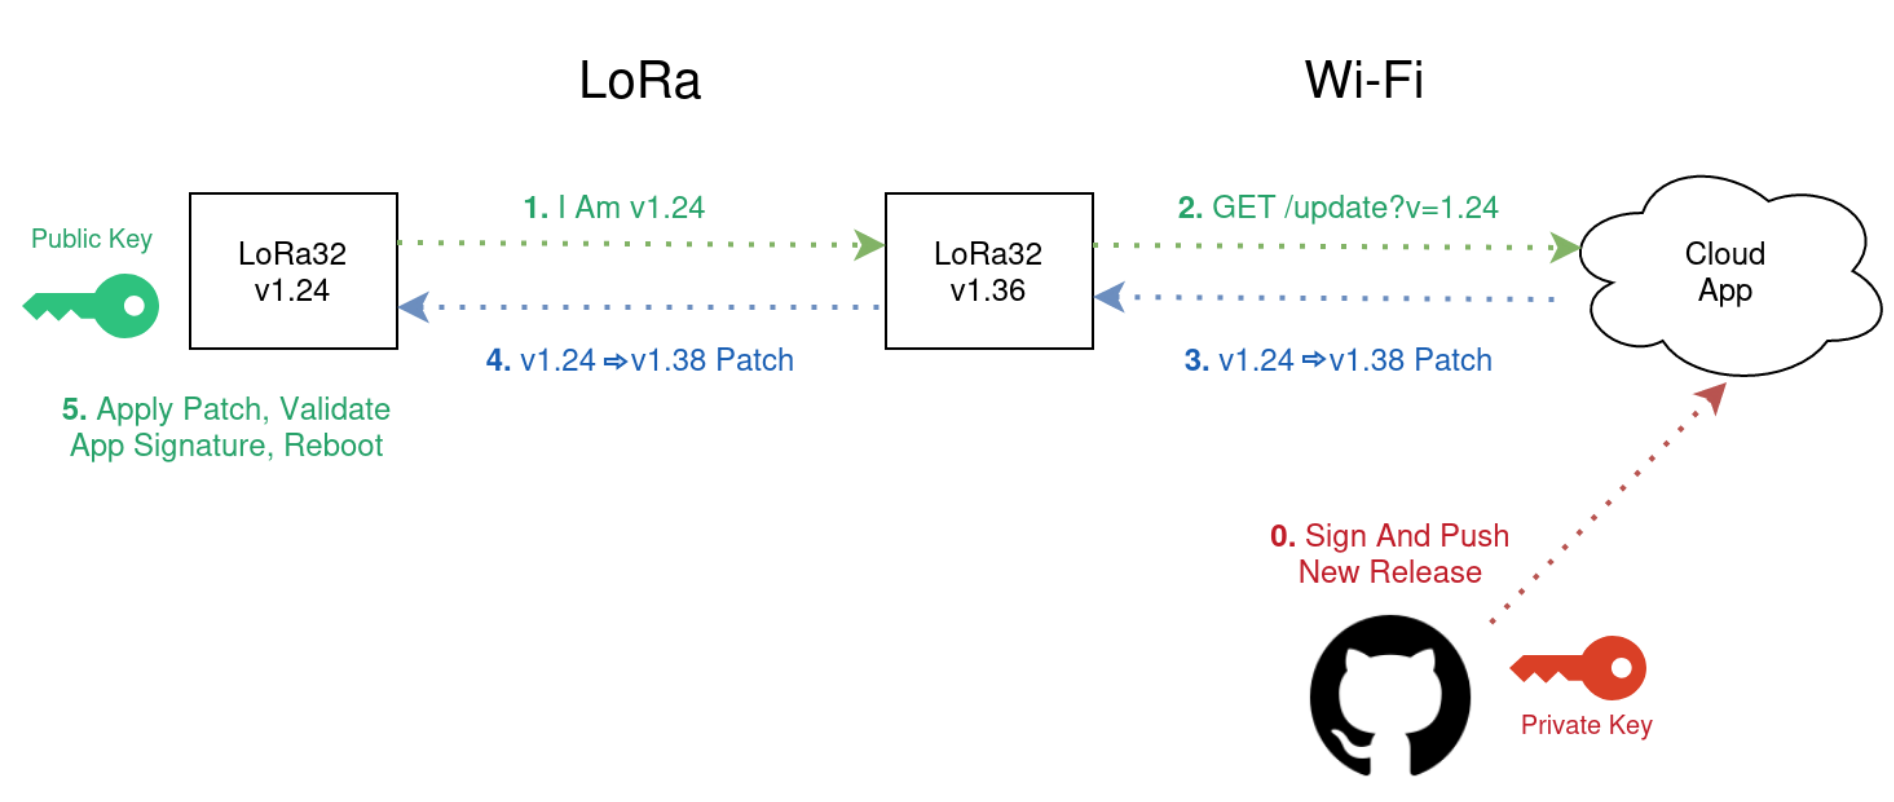
\includegraphics[width=90mm]{images/updates.png}}
\caption{System architecture diagram detailing the procedure used to securely update the firmware of sensor devices remotely}
\label{updates_figure}
\end{figure}




\section{LoRa Communication} \label{lora}

While I have not had much role in configuring the LoRa module and selecting radio parameters to optimise for range, which has primarily been left to Emmet Morrin and Cian Mawhinney, I have spent some time examining the LoRa communication protocol we use to facilitate the publication of synchronised bang timestamp publication and the reception of OTA firmware updates within the bang sensor network. For reference, table \ref{packet_table} defines the structure of each packet type mentioned. A description of their design and purpose within the implemented protocol is provided in the following sections.

\begin{table}[ht]
\caption{128 Bit LoRa Packet Type Structures}
\begin{center}
\begin{tabular}{|c|c|c|}
\hline
\textbf{Label} & \textbf{Bits 0:63} & \textbf{Bits 64:127} \\
\hline
\textit{sync} & Time Reference & OTA Version \\
\hline
\textit{bang} & Sensor Identifier & Timestamp \\
\hline
\textit{ping} & Sensor Identifier & Version Identifier \\
\hline
\textit{ota} & OTA Data & OTA Data \\
\hline
\end{tabular}
\label{packet_table}
\end{center}
\end{table}

\subsection{Bang Timestamp Publication}

\begin{figure}[ht]
\centerline{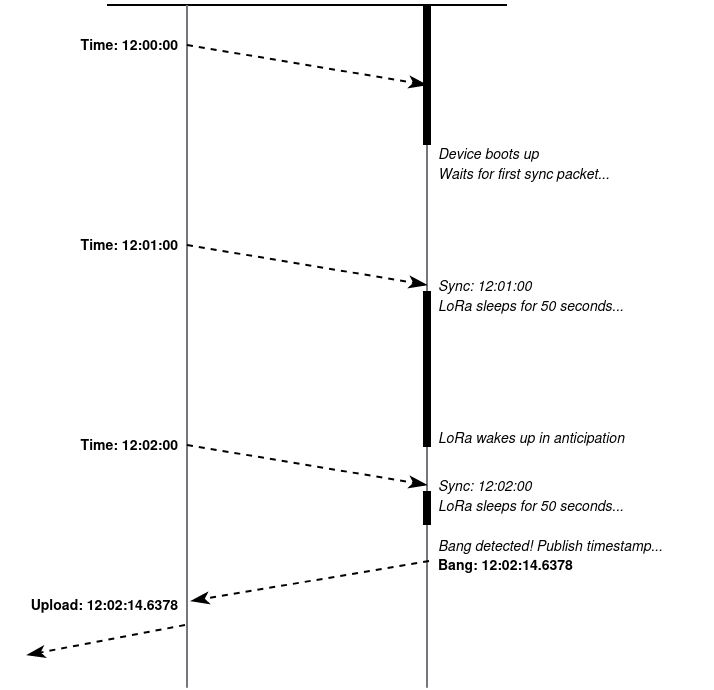
\includegraphics[width=90mm]{images/ping.png}}
\caption{Network sequence diagram describing time synchronisation}
\label{ping_figure}
\end{figure}

In order for sensor timestamps to be synchronised with the time reference known to the gateway through NTP, gateway sensors regularly broadcast a `sync' packet containing the current time reference as a 64 bit timestamp. Once a remote sensor device is booted up, it will begin listening for these packets to synchronise its time with. To reduce power consumption, after the remote sensor device has been first synchronised, it will use receiver windows by placing LoRa module into a sleep mode until a few seconds before it anticipates the next `sync' packet from the gateway. Once again, it will listen for a `sync' packet and then return to the LoRa module to sleep.

A remote sensor device which has been synchronised will detect bangs, associate the bang with the current time and then broadcast this as a 64 bit timestamp within a `bang' packet. This `bang' packet also contains a 64 bit identifier for the sensor device, totalling 128 bits. When the gateway receives such a packet, it uploads this information to our cloud application using the HTTP API.

\subsection{OTA Firmware Updates}

\begin{figure}[ht]
\centerline{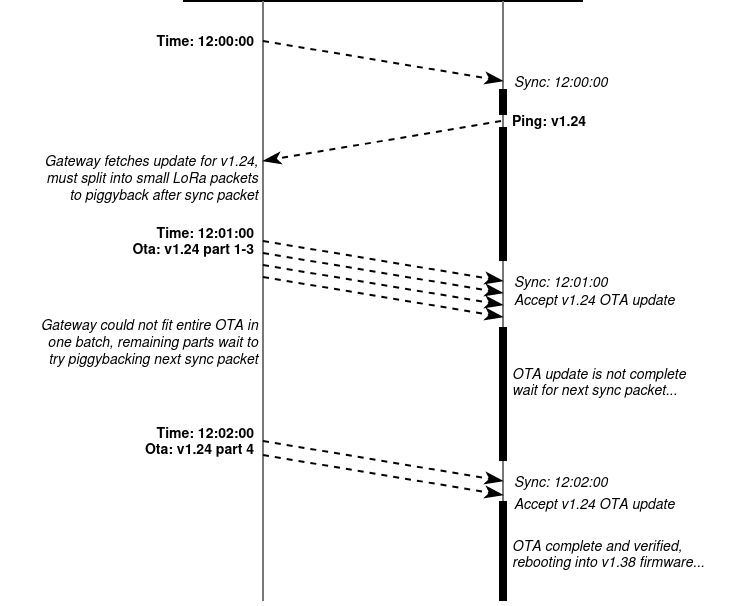
\includegraphics[width=90mm]{images/ota.png}}
\caption{Network sequence diagram describing OTA updates}
\label{ota_figure}
\end{figure}

To allow for delta-encoded OTA firmware updates as explained in section \ref{updates}, remote sensor devices also regularly, but at a much lower frequency, broadcast a `ping' packet containing their 64 bit identifier for the sensor device and a 64 bit identifier for the current firmware version. Gateway devices which receive this packets will query our cloud application API for an appropriate binary patches, if any, and then queue the patch for broadcast during the next receiver window.

As the receiver window on all remote sensor devices occurs in anticipation for the next `sync' packet and we want to send OTA data without transgressing LoRa duty cycles, the `sync' packet also includes the version identifier for the OTA binary patch the following OTA packets apply to. This field is zeroed out if there are no packets to follow. Then up to 4 `ota' packets are sent, each containing the next 128 bits of OTA binary patch data. In this way, the `ota' packets ``piggyback'' on the transmission of the `sync' packet. Eventually, all of the patch data is received by the appropriate remote sensor devices which can then verify the integrity and authenticity of the update using our public key against the provided signature within the update before rebooting.


\section{Conclusion}

To summarise the work completed so far within my areas of responsibility, we have a working build pipeline using the Arduino framework as an ESP-IDF component with FreeRTOS asynchronism, each device's time reference is synchronised across the bang sensor network using NTP and LoRa, secure remote firmware updates are facilitated using ESP-IDF OTA with Signed App Verification, and our bang sensor network communication protocol for accurate bang timestamp publication has been demonstrated to function on top of LoRa without issue at distances up to 510 metres. Yet to be completed is full integration with our projects cloud component as well as the automated generation of binary firmware patches to be applied to out-of-date firmware on remote devices.

Looking back on the project as a whole, while our team did properly consider the requirements and tasks needed to reach our goal, I feel it would have been greatly beneficial for us to have taken the time to plan out the entire development timeline before jumping straight into the first weekly sprint. With no fixed deadlines for features outside of just the current week's tasks, we are left without firm understanding of our overall progress and which areas we need to prioritise. This is not to say we are not progressing, only I would be more confident in our abilities if we could compare ourselves to a carefully considered schedule. I should point out a merit of our methodology does allow us to remain more adaptive in the event of setbacks or pivots, but this project has been concise enough for us so far to not suffer from these.

I also regret not spending time comprehensively investigating PlatformIO before permitting our team to begin development on our prototype with it. This resulted in a number of wasted hours and somewhat disjointed development as we later needed to migrate our codebase to ESP-IDF when it was discovered that PlatformIO did not support Signed App Verification. Such an outcome could have been entirely avoided had I only taken a cursory glance at how Signed App Verification was enabled and whether our chosen build tools would provide the flexibility to do so. This would have become apparent during the production of minimal demonstrations for usage of the build tool in the context of our project requirements. In the future, to reduce the possibility of choosing inadequate tooling, I will devote more effort to initial research and testing of required functionality.

\printbibliography

\end{document}
